% Chapter 4

\chapter{Design and Implementation} % Main chapter title

\label{desi} % For referencing the chapter elsewhere, use \ref{desi}

\lhead{Chapter 4. \emph{Design and Implementation}} % This is for the header on each page - perhaps a shortened title

%----------------------------------------------------------------------------------------
\section{Definition of gamification strategy}

The primary design decision to start the gamification process was the integration of a casual game within AnkiDroid. It was motivated for two reasons, first, casual games are simple and their gameplays allow to play them over short periods of time. These characteristics make casual games activities that can be executed during work or study breaks. In these conditions, AnkiDroid users could switch from reviewing cards to playing the game during breaks. However, the main reason to integrate a casual game was the setting of an stage to add game components into AnkiDroid. Therefore, it was necessary to establish a connection between AnkiDroid and the game which required modifying the latter.

%----------------------------------------------------------------------------------------
\subsection{Modifications of the game}
The selected game was 2048 \citep{uberspot2017game}. It is a puzzle type game with a 4x4 grid as seen in Figure \ref{fig:2048-grid}. The objective of the game is to merge numbered blocks until create one with the value 2048. The game starts with two blocks of value 2 which are randomly positioned in the grid. The player has to slide the blocks horizontally or vertically. The blocks move in the choosen direction; a block stops if it reaches an edge of the grid or collides with another block. If two colliding blocks have the same number, they are merged into a single block which value is the sum of the values of the forming blocks. In every turn, a new block of value 2 is randomly positioned in the grid.

\begin{figure}[htb]
    \vskip 5mm
        \begin{center}
            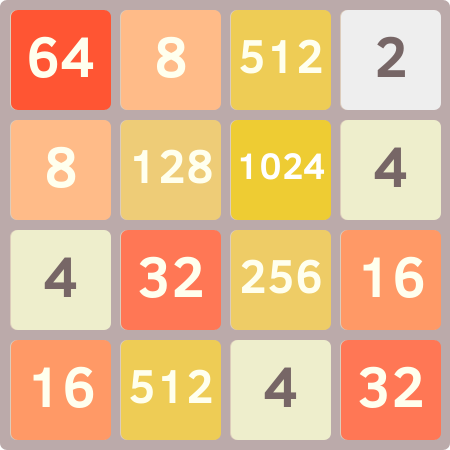
\includegraphics[scale=0.5]{./Figures/game_grid.png}
            \caption{Grid of the 2048 game.}
            \label{fig:2048-grid}
        \end{center}
    \vskip -5mm
\end{figure}

The game is simple, yet challenging due to the high number of turns to form the block 2048 (1024 turns in the perfect case). Another aspect that increases the difficulty of the game is the limited space, if there exist no more empty cells in the grid, and no further movements are possible, then the game is over. These conditions set a perfect scenario to modify the game and reduce its diffculty. Such modifications have to be consistent with the easy-to-use paradigm of casual games. Moreover, they need to mantain a consistency among them such that the usage and results of all of them are similar.

Based on the requirements for the modifications of the game, they were implemented in the form of cheat tricks. These tricks were meant to reduce the difficulty of the game by altering the state of the grid. The state of the grid is defined by the positions of the blocks and their values at a given turn. Therefore, there exist several options to change the state of the board. Moreover, each possible cheat trick needs to provide a different degree of benefit, thus, they're not equally valuable. The modifications included four cheat tricks as seen in Table \ref{tab:tricks}. It is important to note the restrictions in their usage based on the state of the grid.

\begin{table*}[!htb]
	\centering
	{\renewcommand{\arraystretch}{2}
		\begin{tabular}{|R{2cm}|R{6cm}|R{5cm}|}
		\hline
		\multicolumn{1}{|>{\centering\arraybackslash}m{2cm}|}{\textbf{Name}} &
		\multicolumn{1}{>{\centering\arraybackslash}m{6cm}|}{\textbf{Benefit}} &
		\multicolumn{1}{>{\centering\arraybackslash}m{5cm}|}{\textbf{Usage conditions}}\\
		\hline
		Gift & Adds a randomly positioned block that can merge with any block which value is less than 512. & There is at least one empty cell in the grid.\\
		\hline
		Doubler & Doubles all the blocks which values are 2. & There is at least one block of value 2 in the grid.\\
		\hline
		Remover & Removes all the blocks which values are 2. & There is at least one block of value 2 in the grid. \newline There is least one block of value greater than 2.\\
		\hline
		Undo & Undoes the last movements (up to 10 previous movements). & There are previous movements.\\
		\hline
		\end{tabular}
	}
	\caption{Cheat tricks for the game, their benefits, and usage conditions}
	\label{tab:tricks}
\end{table*}

%----------------------------------------------------------------------------------------
\subsection{Resources}
Once the game modifications were ready, game elements in AnkiDroid started to be added. The next important design decision was aimed to allow users obtain the benefits of tricks in exchange of something. This is something common in games where users buy assets and other elements using a virtual currency. In some cases, the virtual currency is mapped to a real one. However, a simpler approach requires the user to do some activities within the game to earn virtual money. Following this scheme, the decision led to the implementation of game coins as the resource to be exchanged for tricks. Unlike games, the users are not required to do activities in the game but within AnkiDroid to earn game coins.

In addition to doing activities to earn coins, the main interest is to keep users motivated to use AnkiDroid features. Moreover, one of the most relevant features of the application is the revision of flashcards. These three conditions set a suitable scenario to allow the users earn coins. Thus, game coins were defined as a resource to be obtained as a result of reviewing cards which converted them in the first motivational element to increase user engagement. The premise is that the more cards a user reviews, the higher the number of earned coins. This simple rule needed to consider some relevant aspects about the revision process to avoid unexpected behaviours from the users.

The revision process of flashcards has two components. The first one is the displaying of the front of the flashcard (or question); the second one is the exhibition of the back of the flashcard (or answer) followed by the corresponding difficulty assessment. After a flashcard is assessed a new question is automatically displayed to the user, repeting the process indefinitely. From the user's perspective there are two moments for each card: watching the question and revealing the answer. In both moments the user needs to interact with the application to continue to the following one. This means that the user decides how much time questions and answers are displayed. However, the time for each flashcard greatly depends on its content.

The content of flashcards varies from deck to deck, it can be as simple as text, or as complex as including multimedia components like images and audio. The other aspect that defined the amount of time per flashcard is its easiness which is defined by the user. Both conditions mean that there is a correlation between the time to review a flashcard and the users' effort. Under this condition, it is fair to define the number of coins per flashcard as a function of time. However, a couple of restrictions had to be considered to avoid undesired behaviours from users.

The first undesired behaviour is passing flashcards as fast as possible to obtain the highest number of possible coins. Another behaviour is spending more time than needed to review flashcards to obtain more coins in each flashcard. The strategy to diminish these behaviours consisted in the setting of ranges of time when seeing questions and answers. Therefore, there are three ranges to calculate the number of coins in each card: null, linear, and constant. In the null range no coins are given, it lasts for one second from the moment a question or an answer are displayed. The linear range lasts for three seconds; here, the number of coins are proportional to the amount of time. Finally, in the constant range no further coins are given; it lasts until the user display the answer of the card of a new question.

\begin{equation}
	c(t) =
  		\begin{cases}
  			0 & \text{if t $\leq$ 1}\\
  			t & \text{if 1 $<$ t $\leq$ 3}\\
  			3 & \text{if t $>$ 3}\\
  		\end{cases}
  	\label{eq:coins-formula}
\end{equation}

The described formula to calculate coins is shown in Equation \ref{eq:coins-formula}, where \textit{c} is the number of coins and \textit{t} is time in seconds. If the number of coins has a decimal part, then it is rounded to the closest integer. It is important to note there is a minimum and maximum number of coins that can be earned in each card, 0 and 6 respectively. A potential drawback when calculating coins is the repetition of a card. AnkiDroid allows to undo the previous reviewed flashcard so that a user can earn additional coins in a single flashcard. However, reviewing the previous flashcard again should not be penalized. Therefore, the previously earned coins are kept. It is worth to remember that the flashcards are shown to users based on how they assess them, thus, AnkiDroid can display them repeatedly in a short period of time.

%----------------------------------------------------------------------------------------
\subsection{Rewards}
Since coins are given after reviewing a card, they can be seen as a reward as well. However, their dynamic characteristic (they can be spent by the user), and how they are calculated reduce their potential benefits as rewards. Thus, it was necessary to implement a new element with a similar earning scheme but different characteristics. Points are a common element in games, their objective varies from context to context, but usually they provide information about progress. Other educational platforms have added points as motivational element \citep{disalvo2014khan}.

Points were designed to be calculated in a similar way to coins. Similarly, there exist ranges of time to earn coins. The first range has the same objective as the one for coins, therefore, its duration is similar. A second range is meant to earn coins proportionally to the time, however, the relation is not linear but logaritmic as seen in Equation \ref{eq:points-formula}, where \textit{p} is the number of points and \textit{t} is time in seconds. Since logaritms are negative for values less than one, a max function between 1 and the logaritm is applied to avoid negative points. If the number of points has a decimal part, then it is rounded to the closest integer.

This logaritmic relation and the lack of a limit for points have two objectives, the first one is to create an additional distinction between points and games. If the number of coins and points in a flashcard are greater than 0, it is unlikely that they are the same value. The second goal has to do with the limit for coins. Since the content of some flashcards can require more time than usual to review, the maximum number of coins per flashcard acts as a penalization for flashcards with large content. Therefore, the lack of a limit for the number of points earned in a flashcard compensates the coins penalization in large flashcards.

\begin{equation}
	p(t) =
  		\begin{cases}
  			0 & \text{if t $\leq$ 1}\\
  			max(1, 10log(t)) & \text{if t $>$ 1}\\
  		\end{cases}
  	\label{eq:points-formula}
\end{equation}

The informative characteristic of points was also leveraged to increase the connection between AnkiDroid and the game. There are two considerations. First, using cheat tricks in the game depends on the number of coins i.e. the time spent reviewing cards. In addition, the schemes to earn points and coins is similar. Therefore, it is possible to add another modification in the game based on points. Such modifications is the availability of tricks. This means that tricks are initially blocked. Using cheat tricks requires to earn a given number of points to unblock them. Thus, using a cheat trick requires to fulfill three conditions: required number or points to unblock it, required number of coins to buy it, and no restriction as seen in Table \ref{tab:tricks}.

%----------------------------------------------------------------------------------------
\subsection{Social and competition}
The informative nature of points can also be used to integrate other common element to games: a leaderboard. This component has two objectives, first, it provides a social context to the users. Thus, users know that there are other people using the application. The second objective is the sense of competition which add another motivational aspect to the revision of flashcards. Even though users of the application can not directly communicate to each other, and it is likely they do not have any kind of relationship among them, they are able to see the progress of each other wwen checking the positions on the leaderboard which are set based on the number of earned points of each user.

%----------------------------------------------------------------------------------------
\subsection{Achievements}
Rewards are by nature obtained after doing small tasks. Until this point, the rewards were designed as coins and points to be earned in every reviewed flashcard. However, several games implements more advanced elements that increases the player's motivation. Such elements are known as achievements, which are similar to rewards. The main difference relies in the size of the tasks which are bigger for achievements. Unblocking the cheat tricks in the game can be seen as achievements. However, a further step required to design achievements in the context of AnkiDroid.

Following some game schemes, the achievements in the context of AnkiDroid were defined as ankimals (pets) that have to be rescued. Therefore, an achievement was defined as a task aimed to rescue the ankimals. Similar to cheat tricks in the game, ankimals have an specific order based on the number of required points to rescue them. However, the main difference between cheat tricks and ankimals are the notification aspect of the latter. The user has no feedback when the number of points to unblock a cheat trick has been reached.

The lack of notifications for unblocked cheat tricks is due to the objective of the gamification process. The user has to be motivated to use AnkiDroid not the game. However, since ankimals were defined as achievements based on the number of earned points, it is important to inform the user when an achievement has been reached. For this reason, the design included notifications for the user to inform about the rescued ankimal. The notifications also encourage the user to earn more points, hence reviewing more flashcards, to get more achievements as seen in Figure \ref{fig:ankimals-rescue}.

\begin{figure}[htb]
    \vskip 5mm
        \begin{center}
            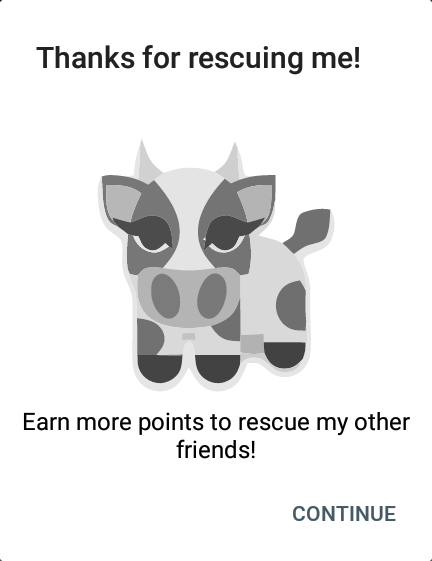
\includegraphics[scale=0.5]{./Figures/achievement_notification.png}
            \caption{Notification shown to user when achievement is reached.}
            \label{fig:ankimals-rescue}
        \end{center}
    \vskip -5mm
\end{figure}

%----------------------------------------------------------------------------------------
\subsection{Customization}
Games provides customization aspects to give a more personal experience to players. Following this idea, two customizable components were designed. The first one was a nickname that can be set by the user. This element gives a higher sense of participation within the application. The second aspect for a custom experiences are avatars. Avatars are meant to provide a visual representation of a player which creates a sense of individuality in the user. Taking advantage of the existence of ankimals in the form of images, they were used as potential avatars for users.

Selecting an ankimal as an avatar required two considerations. The first one is related to coins. As seen previously, the objective of coins was to buy cheat tricks in the game. A potential problem of this design is the lack of interest of users in the game. Thus, coins can become an idle resource. Diminishing this problem required to find additional assets to be acquired in exchange of coins. Since, rescued ankimals were originally represented as grayscale images, they become suitable elements for the use of coins. Therefore, ankimals were designed to be colored and set as avatars in exchange of coins. Finally, to complement the social and competitive aspect of the leaderboard, the nickname and the avatar of every player were displayed in the leaderboard.

%----------------------------------------------------------------------------------------
\subsection{Progress}
Other important components of games are the visual elements that give information about progress and other aspects. This scheme was designed in the application as a status bar that displayed information about points, coins, rescued ankimals, avatar and nickname. The status bar was set to be displayed in the most relevant screens of the applications: deck picker, reviewer, and game. Additionally, a list of the ankimals was also added in the deck picker to show the rescued and not rescued ankimals. This list was also set to allow the selection and coloring of the ankimals.

%----------------------------------------------------------------------------------------
\section{User interface considerations}
Several user interface aspects were considered to implement the game elements described earlier. First, the modifications in the game required the addition of interactive elements for each cheat trick. Initially, color information was used to differentiate the cheat tricks and to provide clues about their status (blocked, enabled, usable). Moreover, since the gameplay of the game required the users to slide vertically and horizontally, cheat tricks could easily be selected by mistake. Avoiding that problem required to design a traslucent curtain to be removed by the user before selecting cheat tricks.

In AnkiDroid, the main considerations to implement the game elements were related to keep consistency in the overall aspect of the application and the visual clues for the user. The first aspect required to use the same color scheme along with other elements like the font type and size. On the other hand visual clues were meant to provide information about modifications in the game elements. This was done by implementing animations where necessary. For instance, when the number of coins or points changed, animations that updated the corresponding visual elements were implemented. Finally, the visual structure was maitained as much as possible to avoid the new components to be intrusive.

%----------------------------------------------------------------------------------------
\section{Data collection}
It was necessary to collect data from the application to analyse it and evalute the effectiveness of the gamification strategy. Originally, AnkiDroid collects a lot of usage information which is presented to users as statistics. These data give users a perspective about their progress based on the number of flashcards review, the number of sessions, the amount of time in sessions and more. The application even forecasts the number of flashcard to be reviewed in the near future. Even though the availability of this type of information, it is not used to evaluate the strategy because it provides a general overiew of the usage from the perspective of users, and discards many details.

\subsection{Types of information}
The information collected in the original application also lacks details related to the integrated game and the gamification elements. Therefore, it was necessary to collect information relevant and specific to the implemented gamification strategy. This information is generated in points where the user interacts with the application like playing the game or reviewing flashcards. There, the users do specific actions that can provide clues about their behaviours and reason about them. The collected information can be grouped into four categories as seen in Table \ref{tab:info-type}.

\begin{table*}[!htb]
	\centering
	{\renewcommand{\arraystretch}{2}
		\begin{tabular}{|R{3cm}|R{6cm}|}
		\hline
		\multicolumn{1}{|>{\centering\arraybackslash}m{2cm}|}{\textbf{Type}} &
		\multicolumn{1}{>{\centering\arraybackslash}m{6cm}|}{\textbf{Description}} \\
		\hline
		Common & Details of time and user.\\
		\hline
		Game & Details about the game.\\
		\hline
		Gamification & Details of game elements. \\
		\hline
		Anki & Details of flashcards and decks. \\
		\hline
		\end{tabular}
	}
	\caption{Types of information collected from the application}
	\label{tab:info-type}
\end{table*}

The first type of information is categorized as common. These data are meant to identify the time, date and user that generate them; they are recorded in every relevant interaction of the user with the application. The next type of information is related to the game; it includes details about the score, cheat tricks, and state of the grid. Game information can provide insights about the effectivenes of the integration. The gamification category has to do with the added game elements to AnkiDroid, it includes details about the number of coins, number of points, and names of the ankimals. Finally, the anki category refers to details about the decks, flashcards, and revision times.

\subsection{Type of logs}
The previously described types of information were stored in the form of logs. The logs are highly linked to the actions done by the users. For this reason, the number of types of logs is bigger than the number of types of information. Nonetheless, the logs can be grouped into two main classes: game logs and anki logs. Games logs are those containing the game type of information, however, some data from the gamification type of information is registered in these logs. Anki logs contain primarily anki type of data with some data of the gamification type. Common type of information is recorded in both groups of logs.

Specifically speaking there are 6 types of game logs and 9 types of anki logs as shown in Table \ref{tab:log-types}. Game logs are expected to be generated in the game context. Something similar occurs with anki logs, however, the design of the solution allows one anki log to be generated in the game context: Check leaderboard. This is possible because user can open the leader-board either in the game context or in the anki context. The reason for this design is that the leaderboard provides information of social aspect. Despite the fact that the leader-board display gamification data (points), users are not asked to do an specific action in anki or the game contexts to see their positions.

\subsection{Storage}
The logs are stored remotely using Fireebase which provides a NoSQL realtime database service. In addition, Firebase provides an analytics service that gives information about usage through standard events automatically generated by the application.
